
% SOURCE docs/release/2026-10-29/source/docs/writing-repair/2026-10-29/src/715d8b709beaf962.tex CHAR 0
\chapter{Discovery, graph uncertainty and identification across models}
\label{r3:discovery}
\section{Define the economic relationships before searching for them}
A bank might supply monthly balances, offered rates, accepted products,
customer contacts and arrears to a discovery procedure. A graph over these
columns is not yet a graph over economic mechanisms. The offer precedes
acceptance, balances are stocks measured at particular dates, arrears affect
eligibility, and a relationship manager may use private information. The
same table can therefore be compatible with several latent-variable and
observation models. The variables, information dates and interventions in
Section~\ref{r3:graph-construction} must be defined before the statistical search.

The output to be learned must also be specified. A DAG with no hidden
common causes, a Markov equivalence class of such DAGs, a latent projection,
and an equivalence class of ancestral graphs encode different information.
Changing a graph's serialization without preserving its class can change
the identification argument even when its visible arrows look identical.
Discovery is useful because it can reject some scientific specifications,
suggest missing variables and narrow intervention questions. Its strongest
conclusion remains conditional on the model class and discovery assumptions.

\section{From a full DAG to observed mixed graphs}
\label{r3:latent-graphs}
Let the full acyclic causal graph have observed vertices $V$ and hidden
vertices $U$. One observed-variable representation is an acyclic directed
mixed graph (ADMG). A directed edge $X\to Y$ in a latent projection can
summarize a directed path with hidden internal vertices; a bidirected edge
$X\leftrightarrow Y$ can summarize a path with arrowheads at both
observed endpoints and hidden noncolliders internally. Directed cycles
remain excluded, but a directed and bidirected edge can coexist between
the same pair. For example, $A\to Y$ together with $A\leftarrow U\to Y$
gives the bow $A\to Y$, $A\leftrightarrow Y$. Its two marks retain both
causal transmission and confounding. Districts connected by bidirected
edges are the objects used by the ID decomposition of
Section~\ref{r3:id-algorithm} \citep{id2006}.

A maximal ancestral graph (MAG) used for conditional-independence discovery
is a different representation. In the no-selection setting, it has directed
and bidirected edges, no directed or almost-directed cycles, and every
nonadjacent pair can be separated by other observed vertices. An arrowhead
at $X$ on an edge to $Y$ rules out $X$ being an ancestor of $Y$. The bow
above is therefore not an ancestral graph. Its MAG on just $A,Y$ is
$A\to Y$, which records ancestry but can still represent hidden confounding.
Interpreting that MAG as a causally sufficient DAG would incorrectly
license adjustment by the empty set.

\citet[Section 3, Definitions 1--3]{zhang2008} gives the construction.
Join two observed vertices if there is an \emph{inducing path} in the full
DAG: every observed internal vertex is a collider and every collider is
an ancestor of an endpoint. Hidden internal noncolliders are allowed.
Orient the resulting adjacency by ancestry in the original DAG: a tail
at an ancestor and an arrowhead at a nonancestor. If neither endpoint
is an ancestor of the other, use two arrowheads. This construction
preserves the marginal conditional independences and observed ancestry;
it does not uniquely recover the latent DAG or every intervention law.

\subsection{Separation and endpoint semantics}
On a mixed-graph path, a collider has two incident arrowheads pointing
into it. A path is $m$-connecting given $Z$ if each noncollider is outside
$Z$ and each collider is an ancestor of a member of $Z$, including itself.
The endpoints are $m$-separated if there is no such path. This extends
$d$-separation without changing the reason conditioning on a collider
can open a path \citep[Definition 2]{zhang2008}.

A completed partially directed acyclic graph (CPDAG) represents a DAG
Markov equivalence class. Its directed edges have that direction in every
member; its undirected edges can vary across compatible DAGs. DAGs are
Markov equivalent exactly when they share a skeleton and unshielded
colliders \citep[Definition 6.24, Lemma 6.25]{peters2017}.
A partial ancestral graph (PAG) represents a MAG equivalence class.
An invariant arrowhead or tail appears at the corresponding endpoint;
a circle means that endpoint mark varies across represented MAGs.
For example, $A\mathbin{\circ\!\!\to}Y$ establishes that $Y$ is not
an ancestor of $A$, but leaves the status at $A$ unresolved. It does
not say that $A$ is definitely a cause of $Y$. Nor do endpoint circles
vary independently: allowed completions must satisfy the whole graph's
ancestral and equivalence constraints \citep[Definition 3]{zhang2008}.

These definitions exclude selection variables. General ancestral graphs
can also contain undirected edges encoding selection structure. A bank
sample restricted to approved borrowers or surviving accounts cannot
inherit a no-selection theorem merely by removing the selection column.
An ADMG causal model may also imply observable restrictions beyond
conditional independence; learning its MAG does not preserve all of that
structural information. This is one reason to retain an assumed economic
model alongside, and separately from, a discovered equivalence graph.

\section{Conditional independence: oracle logic and finite information}
\label{r3:pc-fci}
Under causal sufficiency, the causal Markov property makes graphical
separation imply independence. Faithfulness supplies the converse.
With a perfect conditional-independence oracle, the PC procedure starts
with a complete undirected graph and removes $X-Y$ when it finds
$X\perp Y\mid S$. Searching growing subsets of current neighbors
uses the fact that nonadjacent DAG vertices can be separated by the
parents of one endpoint. It stores each separating set. For an
unshielded triple $X-M-Y$ with $X,Y$ nonadjacent, $M\notin S_{XY}$
identifies the collider $X\to M\leftarrow Y$ under the oracle
assumptions. Orientation rules then avoid new unshielded colliders
and directed cycles and propagate compelled directions
\citep[Sections 2.2--2.3]{kalisch2007}.

With latent variables, observed parents need not supply all required
separators. FCI adds searches over possible separating sets and uses
ancestral-graph orientation rules, returning a PAG under its assumptions.
Simply relabelling PC's undirected output a PAG does not perform that
search. The latent and time-window issues in
\citet[Section 2]{gerhardus2020} build on this distinction; the MAG/PAG
semantics and oracle interpretation are made explicit in
\citet[Section 3]{zhang2008}.

The oracle argument is not finite-sample certification. Failing to reject
a conditional-independence null does not establish independence. Testing
many adaptively selected conditioning sets can create incompatible
separating statements. Sparse graphs reduce the number and size of the
sets, but variables that are almost deterministically related can make
both estimation and testing unstable.

\subsection{The signal restriction behind high-dimensional recovery}
Theorems 1--2 of \citet{kalisch2007} concern independent Gaussian
vectors, not arbitrary nonlinear time series. Their assumptions allow
$p_n=O(n^a)$ variables and maximum degree $q_n=O(n^{1-b})$, with
$0<b\le1$. Nonzero relevant partial correlations have magnitude at
least $c_n$, where $c_n^{-1}=O(n^d)$ for $0<d<b/2$; absolute partial
correlations are uniformly below some $M<1$. With a suitable vanishing
test level, the recovered CPDAG is correct with probability
$1-O\{\exp(-Cn^{1-2d})\}$. The lower signal bound is a substantive
restriction on how rapidly an apparent independence may be approached.
The result is not a guarantee for a fixed test threshold on millions of
weakly dependent banking variables.

To see the issue without asymptotics, take independent centered Gaussian
noise and the SCM
\[
 A=\epsilon_A,\qquad M=A+\epsilon_M,\qquad
 Y=M-A+\epsilon_Y=\epsilon_M+\epsilon_Y.
\]
The graph contains $A\to M$, $M\to Y$ and $A\to Y$, but $A\perp Y$.
The direct and indirect paths cancel. Replacing the direct coefficient
$-1$ by $-1+\delta$ makes their marginal covariance arbitrarily small.
More data helps distinguish a fixed nonzero $\delta$; it does not give
a uniform separation guarantee over arbitrarily small signals. A
stability frequency from resampling is useful evidence about this
algorithm and data regime, but is not a posterior probability that a
causal arrow exists.

\section{Scores and functional restrictions supply different information}
\label{r3:discovery-scores}
A score-based search minimizes a penalized negative log-likelihood over
graphs. If the score is equivalent across Markov-equivalent DAGs, the
likelihood cannot choose their directions. A Bayesian prior or a
deterministic tie-break can choose a representative, but that choice
must not be presented as observational identification.

For a linear coefficient matrix $W$, the NOTEARS constraint is
\begin{equation}
 h(W)=\operatorname{tr}\{\exp(W\circ W)\}-d=0,
 \label{r3:notears}
\end{equation}
where $\circ$ denotes elementwise multiplication. Write $B=W\circ W$.
The series $h(W)=\sum_{k\ge1}\operatorname{tr}(B^k)/k!$ has
nonnegative terms; a directed cycle contributes a positive product to
a diagonal entry of one power. Conversely, a DAG can be permuted to
strict triangular form, so every power has zero diagonal. This proves
the acyclicity equivalence in \citet[Theorem 1]{notears2018}.
It proves a property of the feasible matrix, not causal sufficiency,
global optimization, or uniqueness of the causal graph. A loss based
on unweighted squared residuals additionally privileges a noise scale;
rescaling currency and ratio variables can change that comparison.

Functional-model methods restrict mechanisms more strongly than Markov
and faithfulness assumptions. For $Y=f(X)+\epsilon_Y$ with
$\epsilon_Y\perp X$, a reverse additive-noise representation need
not exist. But both directions do exist in the bivariate linear
Gaussian case: each regression residual is Gaussian and independent
of its regressor. Non-Gaussian independent noise with an acyclic
linear system supplies additional information through ICA; the
structural VAR construction in Chapter~\ref{r3:time-series} uses
that information \citep[Sections 2.2--2.3]{hyvarinen2010}.
Nonlinear additive-noise identification also needs restrictions
excluding its exceptional reversible cases
\citep[Sections 7.1.2--7.1.5]{peters2017}.

The tradeoff is practical. A conditional-independence method may leave
an equivalence class, while a restricted functional model identifies
a direction if its noise and function assumptions are appropriate.
Neither a neural function approximator nor a small acyclicity loss
can supply evidence for independent disturbances. Residual independence,
sensitivity to variable transformations, held-out model adequacy and
alternate graph classes are therefore relevant diagnostics. Passing
them leaves the substantive assumptions conditional.

\section{Temporal discovery must preserve the clock and hidden history}
\label{r3:temporal-discovery}
For an unrolled process graph, time order can exclude arrows from a
future decision into an earlier outcome. A cycle in the summary graph,
such as balance affecting next month's offer and offer affecting next
month's balance, is compatible with an acyclic unrolled graph.
Instantaneous cycles at the observation scale need a different model;
forcing an arbitrary within-month ordering imposes a restriction.

PCMCI-type methods reduce conditioning sets and test lagged links with
conditions chosen to control autocorrelation and common parents.
PCMCI+ also treats contemporaneous structure.
\citet[Assumptions 1 and Theorems 1--2]{runge2020} requires causal
sufficiency, Markov and adjacency-faithfulness conditions, consistent
CI decisions, stationarity, time order and a maximum lag covering the
true parent lags. Its stated setting excludes selection and measurement
error. Collider-rule choices determine the corresponding completeness
claim. These conditions explain both its usefulness for repeated
mechanisms and why it cannot automatically certify effects from a
monthly table of selected accounts.

LPCMCI permits latent confounders but changes the graph object and
conditioning problem \citep[Sections 2.1--2.3]{gerhardus2020}.
When only a finite lag window is retained, earlier observed variables
are themselves marginalized. Increasing the window can remove edges
\emph{inside} the old window because a previously hidden separator
becomes observed. Thus a maximum-lag choice is partly a scientific
observation choice, not merely a hyperparameter. The primary paper also
distinguishes how stationarity constrains repeating adjacencies and
orientations. Its stationary, acyclic, no-selection model is not a
general theorem for arbitrary missing or irregular event histories.

The subsampling example in Section~\ref{r3:temporal-observation} makes this
restriction concrete: a two-day series cannot distinguish daily
coefficients $0.7$ and $-0.7$. Temporal order does not restore the lost
daily response. Aggregated flows can additionally induce dependent
innovations and change the conditional-independence structure. A
discovery operation must therefore record the observation operator,
lag window, contemporaneous rules and stationarity regime alongside
the returned endpoints.



% SOURCE docs/release/2026-10-29/source/docs/writing-repair/2026-10-29/src/737d1a144d864676.tex CHAR 0
\section{A graph and effect confidence construction on the same data}
\label{s4:graph-confidence}
The preceding equivalence-class argument concerns a population law. A
finite-sample construction can preserve that ambiguity without assuming
that a selected graph is correct. Consider independent observations of
three jointly Gaussian variables $(X,A,Y)$, a positive-definite covariance
$\Sigma$, and the class of linear acyclic structural equations with
independent disturbances. The mean is unrestricted. A supplied ordering
may restrict this class; causal sufficiency is a substantive assumption.
We give a deliberately small, conservative reference construction. It
provides a standard against which faster discovery proposals can be judged.

Use the nine directions
$\mathcal V=\{e_i:1\le i\le3\}\cup
\{e_i+e_j,e_i-e_j:i<j\}$. For each $v$, the sample variance $s_v^2$
has pivot $(n-1)s_v^2/(v'\Sigma v)\sim\chi^2_{n-1}$. Give each
variance a two-sided interval with error $\alpha/9$. The union bound
shows that all nine intervals contain their population quantities with
probability at least $1-\alpha$, without independence between pivots.
Diagonal entries follow directly, and
\[
 \Sigma_{ij}=\{\operatorname{Var}(X_i+X_j)
                     -\operatorname{Var}(X_i-X_j)\}/4
\]
gives interval bounds for off-diagonal entries. The resulting entrywise
box is an outer region: it ignores some joint restrictions and may include
non-positive-definite matrices. Keeping these extra matrices can enlarge
the answer but cannot remove the true covariance on the coverage event.

Enumerate the 25 labeled three-vertex DAGs, or the subset respecting a
declared time order. For each graph, list its $d$-separations. In three
variables these require either $\Sigma_{ij}=0$ or
$\Sigma_{ij}\Sigma_{kk}-\Sigma_{ik}\Sigma_{jk}=0$. Discard a graph
only if interval evaluation of one required equality excludes zero.
This is an outer feasibility test, not proof that every retained graph
has a compatible covariance in the region. It needs the Markov property,
but no lower bound on nonzero partial correlations and no faithfulness
assumption. The true graph cannot be discarded when its covariance is
inside the region.

For a retained graph $G$, regress every node on its parents:
$\beta_{j,\operatorname{pa}(j)}=
\Sigma_{\operatorname{pa},\operatorname{pa}}^{-1}
\Sigma_{\operatorname{pa},j}$. With one parent this is a variance ratio.
With two parents it is a two-by-two inverse, evaluated by interval sums,
products and quotients. If the denominator interval reaches zero, return
an unbounded coefficient interval. Multiply coefficients along every
directed path from $A$ to $Y$ and add the products. Their interval sum
$I_G$ encloses the total intervention derivative for every feasible
covariance in that graph. Return
\begin{equation}
 \mathcal C_{AY}=\bigcup_{G\text{ retained}}I_G.
 \label{s4:graph-effect-set}
\end{equation}
On the single simultaneous covariance event, the true graph is retained
and its true effect belongs to its interval. Therefore
$P(\theta_{AY}\in\mathcal C_{AY})\ge1-\alpha$. This proves finite-sample
coverage under the stipulated Gaussian structural class in exact
arithmetic. There is no additional selection penalty because the same
joint event covers all the subsequent transformations. The union is an
\emph{outer confidence set}, not the sharp population identified set or
a collection of posterior arrow probabilities.

The implementation rounds interval additions, products and reciprocals
outward. Sample variances and chi-square quantiles remain ordinary
floating-point numerical calculations. Thus the program approximates the
mathematical construction; it does not supply formally certified numerical
enclosures of transcendental quantiles. Repeated interval occurrences also
lose dependence and can yield very wide bounds. Semialgebraic optimization
over positive-definite covariances and compatible structural equations
could tighten the result, at a substantially larger computational cost.

\subsection{What the construction teaches a banking decision}
In a Gaussian chain $X\to A\to Y$ with action coefficient $0.7$,
the unordered population law permits effects $\{0,0.7\}$ in this
class. Across 500 samples of size 600, the outer effect set contains the
true effect in all samples, but also contains both zero and $0.7$ in
all samples. Its median width is $21.13$, and 1.8\% of runs have an
unbounded set. A supplied order $X\prec A\prec Y$ identifies $0.7$
in the population; even then the conservative finite-sample set contains
both zero and $0.7$ in 83\% of samples, with median width $10.69$.
Tightening computation or gathering more information has economic value
when these alternatives lead to different decisions.

A hidden-common-cause experiment is more revealing. Its true action
effect is zero, but its observational covariance admits a sufficient
ordered model with effect $0.4$. The returned set misses zero in all
500 runs, even though the covariance region covers the actual covariance
in 94.4\% of samples. Coverage of the observed law cannot validate the
causal model class. For 500 successes or failures, a two-sided 95\%
Wilson interval has an endpoint about $0.9924$ or $0.0076$; the zero
plug-in Monte Carlo standard error at these extremes is not certainty.
A measured common cause, a credible instrument, or randomized assignment
would change the information available for this query. A larger
observational sample alone would not identify which class is appropriate.

\section{A supported temporal class and its intervention image}
\label{s4:temporal-graph-confidence}
For a distinct temporal route, stipulate a stable observed Gaussian
VAR(1), $X_t=FX_{t-1}+u_t$, with independent innovations across dates
and coordinates, no contemporaneous causal edges, and a known lag bound
of one. Each nonzero $F_{ij}$ is a directed lagged edge in the unrolled
graph. These are much stronger structural restrictions than those used
by PCMCI+ or LPCMCI. In particular, diagonal innovation covariance is
partly testable, but its observed fit does not rule out every hidden
causal explanation.

OLS has influence matrix $u_tX_{t-1}'Q^{-1}$, with
$Q=\E[X_{t-1}X_{t-1}']$. These scores are martingale differences
because $u_t$ is independent of the past. Ergodicity gives convergence
of their conditional variance and the Gaussian moments give the
Lindeberg condition, so their normalized sum has a multivariate CLT.
Sample outer products of the fitted scores consistently estimate its
covariance; a serial HAC correction is unnecessary in this specified
model. Bonferroni marginal intervals for the $p^2$ coefficients form
an asymptotic joint box $\mathcal B_F$ with coverage at least $1-\alpha$.
Do not set a coefficient to zero merely because its interval includes zero.
Label that edge ``zero or nonzero''; an interval excluding zero supports
a present edge conditional on this class.

An additive intervention raising coordinate $j$ at date zero by one unit
has response $e_i'F^he_j$. For fixed $H$, interval matrix multiplication
maps $\mathcal B_F$ through $F^0,\ldots,F^H$, retaining a simultaneous
outer band for all these responses. If the true $F$ belongs to the box,
every true response belongs to its image, irrespective of thresholded
edge selections. The box may include unstable matrices, which can widen
long-horizon bounds. Intersecting with a justified stability restriction
is allowed; merely clipping a fitted eigenvalue changes the procedure.

With 1,000 dates and 500 replications, the correctly specified three-variable
experiment has whole-response coverage $0.954$ (Monte Carlo standard
error $0.0094$). An omitted second lag gives zero coverage. Its failure
does not recommend a better confidence threshold: it invalidates the
lag-one structural equation and hence its intervention map. Screening,
lag choice and an observation aggregation must be qualified before this
operation is used. General PCMCI/LPCMCI results remain exploratory in the
initial product unless a separate graph-confidence and effect argument
is supplied. Functional-model discovery can orient additional edges only
by adding the noise/mechanism restrictions discussed above; this small
construction does not turn their optimization output into a confidence set.


% SOURCE docs/release/2026-10-29/source/docs/writing-repair/2026-10-29/src/715d8b709beaf962.tex CHAR 13632


\section{Adjustment over an equivalence class}
\label{r3:general-adjustment}
Suppose the graph is a DAG, CPDAG, or a no-selection MAG/PAG, and the
target is the total effect of $A$ on $Y$. An adjustment set must make
\[
 p(y\mid\doop(A=a))=\int p(y\mid a,z)p(z)\,dz
\]
hold for every compatible causal model, not just for a conveniently
oriented representative. Generalized adjustment makes this requirement
precise \citep[Definitions 1--4, Theorem 5]{perkovic2018}.

A possibly directed path has no arrowhead pointing backward along its
direction of traversal. It is proper relative to an exposure set if
only its first vertex is an exposure. An edge $A\to B$ is \emph{visible}
in a MAG/PAG if graph structure certifies that the relevant latent
confounding explanation is absent. A sufficient configuration is
$V\mathbin{*\!\to}A\to B$ with $V$ not adjacent to $B$; the full
definition also permits a collider path into $A$ whose internal vertices
are parents of $B$. All directed DAG/CPDAG edges are visible by convention.
The criterion has three parts:
\begin{enumerate}
\item Every proper possibly directed path from the exposure to the
outcome starts with a visible edge out of the exposure (amenability).
\item The adjustment variables avoid every possible descendant of a
non-exposure vertex on such a path (the forbidden set).
\item They block every proper definite-status noncausal path from
exposure to outcome. A definite noncollider has an incident tail, or
is the middle of the appropriate unshielded circle-marked triple;
colliders have two incident arrowheads.
\end{enumerate}
The cited theorem is sound and complete \emph{for adjustment} in its
stated graph classes. Failure can mean that a front-door or other
identifying functional is needed, or that the target is not identified.
It does not by itself choose between those conclusions. The visible-edge
condition also explains why the two-node MAG $A\to Y$ cannot be
treated as the corresponding causally sufficient DAG.

\section{From unresolved graphs to effects and useful experiments}
\label{r3:graph-effects}
Let $\mathcal G$ be the allowed graph class and $\mathcal M(G,P)$
the structural models with graph $G$ that produce observed law $P$.
The causal identified set is
\begin{equation}
 \Theta(P,\mathcal G)=
 \bigcup_{G\in\mathcal G}\{\theta(M):M\in\mathcal M(G,P)\}.
 \label{r3:graph-union}
\end{equation}
If each graph identifies a functional $\theta_G(P)$, this reduces to
a union of functionals. If some graph does not identify the target,
replacing its inner set by a regression coefficient is invalid.
The union need not be an interval; reporting its convex hull is a
conservative summary that can conceal gaps.

For an exact Gaussian example, let $(A,M,Y)$ have unit variances and
covariances $(\Sigma_{AM},\Sigma_{MY},\Sigma_{AY})=(1/2,1/2,1/4)$.
It has $A\perp Y\mid M$ and no other pairwise conditional
independence. The CPDAG is $A-M-Y$. The three compatible DAGs are
$A\to M\to Y$, $A\leftarrow M\to Y$, and
$A\leftarrow M\leftarrow Y$. Gaussian regressions supply independent
structural errors for each. The total effect of $A$ on $Y$ is $1/4$
in the first model and zero in the other two. The observed law therefore
identifies the set $\{0,1/4\}$ within this causally sufficient linear
class. An arbitrarily accurate estimate of its covariance does not
decide whether an offer changes the eventual financial outcome.
A credible decision-clock restriction that $A$ precedes $M$ would
orient the first edge; an experiment on $A$ would distinguish these
effect hypotheses. These are additional sources of information.

Sampling error is separate from this structural set. If a graph-set
procedure contains the true graph with probability at least $1-\alpha$,
and a confidence set valid for that true graph misses its target with
probability at most $\beta$, their union construction can have coverage
at least $1-\alpha-\beta$ by the union bound. Obtaining those two
properties is the hard part. In particular, post-selection confidence
intervals for a chosen graph do not supply the second property without
an appropriate uniform or independent-sample argument. A bank report
should distinguish graph uncertainty, nuisance/parameter uncertainty
and uncertainty about the substantive model class.

The useful next experiment is one that changes the decision-relevant
identified set. Resolving an edge that all admissible policies ignore
can have little value. In contrast, a randomized encouragement, a new
predecision proxy, finer timing or a deliberately held-out intervention
environment may distinguish the causal explanations that lead to
different banking actions. The scientific request should name that
distinction and its expected value before a discovery engine ranks
variables solely by edge confidence.

\section{The resulting discovery operation}
A reusable discovery result contains its graph class, endpoint marks,
background restrictions, CI or likelihood assumptions, observation and
time-window definition, statistical tuning and unresolved alternatives.
It can feed adjustment/identification queries over a bounded supported
class. It should return a common functional, a set of candidate effects,
or an explicit unresolved query. These are distinct from returning a
best-fitting DAG. Automated data organization must next preserve the
variables and information sets on which these conclusions depend.

The detailed comparisons now separate three uses of discovery. A fitted
temporal search first supplies order sensitivity conditional on its selected
graph. An ancestral-margin example then checks which hidden-variable graph
object is being evaluated. Finally, a covariance region is mapped into a
latent effect set under explicit structural restrictions. These procedures
answer different questions about the same gap between a graph and a decision.



% SOURCE docs/release/2026-10-29/source/docs/writing-repair/2026-10-29/src/0255f65862a062f5.tex CHAR 0
\section{From multivariate temporal search to a conditional effect query}
\label{s5:discovery}
For deposit pricing, balances, lending and market conditions, a useful
discovery workflow must allow lagged and contemporaneous relations. PCMCI+
uses time order and parent selection to address autocorrelation under causal
sufficiency; its contemporaneous output can retain unoriented edges
\citep{runge2020}. LPCMCI allows hidden common causes within its stated
time-series graphical model. A partial-correlation test supplies a linear
Gaussian conditional-independence test, not generic nonlinear independence.
Stationarity, causal Markov, faithfulness, a sufficient lag window and test
validity remain separate premises. Choosing a flexible test changes sample
requirements and computation as well as the null it tests.

The graphical target is itself a method choice. The temporal ancestral-graph
characterization distinguishes the latent projection on a finite window from
its stationarified representation, with potentially different orientation
information \citep[Sections 4.5--4.6 and Propositions 5.2--5.7]{gerhardus2021}.
Its conceptual complete enumeration may be computationally infeasible, and
the inspected 2021 preprint explains why then-current LPCMCI does not recover
every invariant of the stronger time-series graph class. This is not a
claim about every later version. TS-ICD supplies a distinct ordering of
temporal and contemporaneous search under its stationary SVAR/oracle
assumptions \citep{rohekar2023}. Faster orientation under one graph class
is not evidence of completeness under another. The preserved author versions
and later journal identities are recorded separately.

The selected runtime comparison uses Tigramite 5.2.10.1, PCMCI+ and LPCMCI,
with $\alpha=.01$, six variables, 1,600 dates and a maximum lag of two
\citep{runtime_tigramite_scope}. LPCMCI's conditioning search is capped at
three; this is an explicit computational restriction, so no unrestricted
oracle-completeness claim is made. The generator has stable lagged effects,
two contemporaneous triangular relations and independent Gaussian
innovations. A challenger adds an unobserved autocorrelated common cause
of two series. Another searches only lag one while the true mechanism
retains lag two. All graph endpoint strings, conditional-independence
statistics, $p$-matrices and timings are preserved over 20 repetitions.

\begin{center}\small
\begin{tabular}{lrrrr}\toprule
&\multicolumn{2}{c}{PCMCI+}&\multicolumn{2}{c}{LPCMCI}\\
Regime&Precision&Recall&Precision&Recall\\\midrule
Sufficient, lag two&.993&1.000&.971&1.000\\
Hidden common cause&.865&1.000&.815&1.000\\
Omitted second lag&.980&.929&.917&.929\\\bottomrule
\end{tabular}\end{center}
These are descriptive adjacency comparisons with the observed structural
DAG. In the hidden case that DAG adjacency is not the PAG target, so the
numbers must not be read as PAG accuracy or a ranking of latent discovery
correctness. Recall counts true edges outside the requested lag window;
in-window recall alone is one and conceals the omitted-lag defect. Finite
$p$-values and edge-selection frequencies are not graph-confidence levels.

\subsection{A supported transformation and its preserved uncertainty}
The local effect adapter accepts a supplied sufficient temporal graph with
directed lagged edges and directed or unoriented contemporaneous edges. For
at most seven variables it enumerates contemporaneous topological orders
that preserve directed edges and introduce no unrepresented unshielded
collider, including colliders involving lagged parents. It refuses conflicting,
bidirected and partially ancestral endpoints. This is a bounded sufficient
graph operation, not a general PAG completion algorithm.

For each permitted order fit the declared linear structural equations on a
fresh independent 3,000-date sample:
\[
 (I-B_0)X_t=\sum_{\ell=1}^p B_\ell X_{t-\ell}+\varepsilon_t.
\]
Only parents present in that candidate graph enter each equation. The
companion matrix built from $(I-B_0)^{-1}B_\ell$ propagates an additive
equation impulse $(I-B_0)^{-1}e_a$. Query outcome $j$ at horizon $h$ gives
the corresponding coordinate of the propagated vector. The result contains
each order, stability diagnostic and curve, plus a pointwise envelope.
The tested PCMCI+ sufficient graph admits 180 compatible orders, many
differing only in the order of unrelated variables; these are not 180
distinct causal models. LPCMCI output retaining richer marks is refused
by this adapter. The hidden-cause case is outside its sufficiency model,
not proof that every hidden-variable effect is unidentified.

The output is conditional on the selected graph and linear structural
restrictions. A fresh estimation sample prevents reusing search noise in the
coefficient fit, but does not guarantee the selected graph contains the
truth. Consequently the displayed envelope is structural-order sensitivity,
not a confidence band. The earlier finite covariance-region construction
in Section~\ref{s4:graph-confidence} provides a distinct confidence route
under its own bounded model; its guarantee cannot be attached to this search.

A two-series example makes the remaining decision ambiguity material.
Let reduced-form innovations have covariance
$\left(\begin{smallmatrix}1&.6\\.6&1.36\end{smallmatrix}\right)$ and
autoregression $.5I$. One recursive model has a contemporaneous
price-to-balance coefficient .6; a reverse recursive model fits the same
Gaussian innovation law and gives zero balance response to the price
equation impulse. With 8,000 simulated observations the supported order
envelope at impact is $[0,.6096]$, with approximately geometric propagation.
Neither more observations of that unchanged Gaussian law nor a lower search
threshold chooses the causal direction. A documented timing restriction or
an externally randomized price perturbation would distinguish these models.
If the action decision needs a response above .3, the existing evidence does
not make it robust across the two models. This is an actionable request for
additional information, not a decorative ambiguity label.

The practical hierarchy is therefore PCMCI+ for a defensible sufficient
stationary temporal model, LPCMCI as a hidden-confounding challenger with
retained endpoint semantics, and structural identification/effect sets only
where the query's premises justify them. Increasing lag windows can add
identifying information at the population level but increases finite-sample
conditioning cost. Interventions, reliable prior ordering and additional
measurements should be chosen for the effect ambiguity they resolve. A
large discovery runtime cannot by itself convert a search graph into a
bank policy recommendation.


% SOURCE docs/release/2026-10-29/source/docs/writing-repair/2026-10-29/src/51c5de0d00a649a2.tex CHAR 0
\section{Evaluate the observed margin, then ask a causal question}
\label{s6:ancestral-target}
Hidden common causes can create adjacencies absent from the observed portion
of a structural DAG. Consequently precision against that structural portion
is not a measure of recovering the hidden-variable method's target. A
finite-window construction makes the distinction exact. Observe price,
uptake and balance at dates 0 and 1. At each date an unobserved liquidity
state causes price and balance; price causes uptake, which causes balance.
Each variable and the liquidity state have a persistence edge to date 1.
Independent initial innovations define the beginning of the experiment.
There is no silently discarded infinite past.

For this finite DAG $D$ and observed set $O$, join observed nodes $i,j$ if
no subset of $O\setminus\{i,j\}$ d-separates them in $D$. This gives the
adjacency of its maximal ancestral margin. Put a tail at $i$ when $i$ is an
ancestor of $j$ in $D$, and an arrowhead otherwise. There are no selection
variables, so no undirected selection edges are required. An adjacency with
a tail may represent an inducing path, not a directly observed structural
coefficient. A bidirected edge records neither endpoint being an ancestor
of the other. The relation to latent projection, ancestral graphs and
window boundaries is developed in \citet{zhang2008,gerhardus2021}.

This example has six observed nodes and twelve marginal adjacencies. The
oracle checks every one of the 240 pair/conditioning-set queries twice,
using independent NetworkX and Tigramite d-separation implementations
\citep{runtime_networkx_dynamic}.
They agree on all queries. With the resulting population independence
oracle, LPCMCI recovers all twelve adjacencies and makes twelve correct
definite endpoint claims, leaving twelve circles. Those circles are not
errors against a fully oriented generating MAG: a PAG describes an
equivalence class, and unidentifiable orientations must remain unresolved.
The comparison measures correctness of definite ancestry claims and their
informativeness separately. It does not assert completeness of every
orientation under additional temporal background knowledge.

The finite-data experiment uses 2,500 independent two-period episodes per
replication and unrolls their six nodes into columns. LPCMCI is called with
maximum lag zero on these episode rows; this isolates its latent graph
operation without asserting stationarity across the finite window. The
earlier stationary time-series runs remain separate evidence. Treating this
episode construction as an infinite time-series oracle would be wrong:
longer unobserved history can alter its marginal adjacencies, as the
time-series ancestral-graph analysis explains \citep{gerhardus2021}.

With partial-correlation tests, fixed significance .01 and conditioning cap
four, forty repetitions give mean adjacency precision .9977 and recall
.8313, but mean accuracy of definite endpoint claims only .6605. Conflicting
marks are retained as conflicts, not silently converted to arrowheads or
tails. The strong adjacency precision therefore does not qualify a causal
ordering. In the exact population covariance, some genuinely adjacent pairs
have partial correlations as small as .00123 and .00869 under allowed
conditioning sets. Finite testing can remove such edges and then misorient
others. This supplies a concrete weak-faithfulness difficulty; the oracle
comparison shows that changing the target definition alone does not fix
statistical graph recovery. No favorable significance threshold is selected
after these results. Learned endpoints remain exploratory unless supported
by additional scientific information.

\subsection{An identifiable hidden-variable query}
Take the first-date price $A$, uptake $M$ and balance outcome $Y$ under the
substantive front-door graph $A\to M\to Y$, $A\leftrightarrow Y$.
Assume no direct price-to-outcome path, no unblocked back-door path from
$A$ to $M$, and all back-door paths from $M$ to $Y$ blocked by $A$.
These are stronger restrictions than an arbitrary LPCMCI output. Graphical
identification gives \citep{pearl2009,id2006}
\begin{equation}
 \E[Y\mid\doop(A=a)]
 =\sum_mP(m\mid a)\sum_{a'}\E[Y\mid m,a']P(a').
 \label{s6:frontdoor}
\end{equation}
The first factor identifies the action's effect on the mediator. Conditioning
on $A$ closes the mediator/outcome back door, allowing the second factor to
average the mediator intervention over the original action distribution.
The outer sum composes these interventions because the mediator intercepts
every directed path from $A$ to $Y$. An arbitrary adjustment regression on
$M$ would instead remove the mediated effect.

For an exact binary check, let $U$ be fair binary,
$P(A=1\mid U)=.2+.6U$, $P(M=1\mid A)=.15+.6A$ and
$P(Y=1\mid M,U)=.1+.3M+.4U$, with independent assignment noises.
The observed $2\times2\times2$ probability table is enumerated, not fitted.
Equation~\eqref{s6:frontdoor} recovers the structural contrast
$.6\times.3=.18$, while the unadjusted association is .42. A servicing or
deposit application must justify that all relevant pathways truly pass
through the measured uptake variable; a price's direct cash cost would
violate that exclusion if it were included in $Y$. Financial accounting can
add a known direct cost separately, as in the funding dossier, but cannot
wish away an unknown direct behavioral pathway.

\subsection{An unresolved query and its information requirement}
For an action/outcome pair with unrestricted hidden confounding, compare
two SCMs: $U\sim\operatorname{Bernoulli}(1/2)$ and $A=U$ in both,
with $Y=A$ in one and $Y=U$ in the other. Both produce
$P(A=Y=0)=P(A=Y=1)=1/2$. Their average action effects are 1 and 0.
Thus even an exactly known observed distribution and adjacency do not
identify this query. A larger sample or a preferred completion cannot
distinguish the two models.

Additional feasible randomization, observed action-relevant confounders
with support, a defensible instrument with its own target, or validated
front-door restrictions may resolve a suitably redesigned question. Without
such information the product returns the ambiguity and the requested
additional evidence. It does not turn circles into a recursive order.
Fresh estimation data address reuse of outcomes after graph selection;
they do not make the selected graph causally correct. The hidden-variable
query operation therefore records whether identification comes from an
asserted scientific graph, an invariant equivalence-class conclusion or
an unresolved discovery result.


% SOURCE docs/release/2026-10-29/source/docs/writing-repair/2026-10-29/src/075d0543cfab3dad.tex CHAR 0
\section{From an observed-law region to a latent temporal effect set}
\label{c7:latent-confidence}
A selected ancestral graph does not by itself justify intervention confidence.
The alternative developed here retains a whole declared structural class.
Consider three time-ordered variables: an encouragement $Z$, a later action
$A$ and a subsequent financial outcome $Y$. Independent Gaussian episodes
repeat this finite window. The order is scientific information, not an
orientation learned from the same sample. A longer hidden past, selection or
dependence across episodes requires a new observation-law argument.

For graph $G$, write
\begin{equation}
 X=B_GX+\ell_G U+\xi,\qquad
 \Sigma_G=(I-B_G)^{-1}(\ell_G\ell_G'+D_G)(I-B_G)^{-T},\qquad
 \theta_G=[(I-B_G)^{-1}]_{Y,A}.
 \label{c7:structural-map}
\end{equation}
$U$ is a standard Gaussian latent root, $D_G$ is positive diagonal, and
the time-respecting $B_G$ has possible edges $Z\to A$, $Z\to Y$, $A\to Y$.
The broad class enumerates all eight edge subsets and five latent supports:
none, $ZA$, $ZY$, $AY$ and $ZAY$. Loadings and coefficients have no artificial
finite bounds. The 40 descriptions overlap when coefficients vanish; overlap
is harmless for a union and is not counted as 40 distinct data-generating laws.
Here $\theta_G$ is the coefficient of $A$ in the equation for $Y$ because
there is no later intermediate observed variable in this window.

\subsection{A simultaneous covariance region with a finite-sample argument}
For $n$ independent Gaussian episodes, the variance estimate of a scalar
normal contrast $Q=v'X$ satisfies
$(n-1)\widehat{\operatorname{var}}(Q)/\operatorname{var}(Q)
\sim\chi^2_{n-1}$. The unknown mean disappears through centering.
Use the three coordinate contrasts and both signs of each of the three
coordinate pairs, nine contrasts in total. A two-sided variance interval
with error $\alpha/9$ for each contrast gives simultaneous coverage at least
$1-\alpha$ without assuming independence between the nine statistics.
Polarization then yields, for $j\ne k$,
\[
 \Sigma_{jk}=\tfrac14\{\operatorname{var}(X_j+X_k)
                          -\operatorname{var}(X_j-X_k)\}.
\]
The resulting coordinate rectangle $\mathcal C_\Sigma$ contains the true
covariance on that event. It also contains impossible or non-positive-definite
matrices; retaining them is conservative.

The ideal confidence image is
$\bigcup_G\{\theta_G(p):\Sigma_G(p)\in\mathcal C_\Sigma\}$.
The implemented image enlarges structural feasibility to analytically
tractable necessary restrictions. On the coverage event, the true structure
and parameter remain in this larger set if they belong to the declared class.
This proves outer coverage without claiming sharp identification. A graph is
not removed merely because a local optimizer could not find its parameters.

\subsection{Why an unrestricted latent answer can be the whole line}
There is a constructive witness, not just a numerical timeout. For any observed
positive definite covariance, regress $A$ and $Y$ on $Z$ and let their residual
variance/covariance be $v_A,v_Y,c$. For any proposed effect $b\in\mathbb R$,
choose $B_{A,Z}=\Sigma_{ZA}/\Sigma_{ZZ}$ and
$B_{Y,Z}=\Sigma_{ZY}/\Sigma_{ZZ}-bB_{A,Z}$. The two structural residuals
then have covariance $w=c-bv_A$ and variances $v_A$ and
$v=v_Y-2bc+b^2v_A$. Their determinant is
$v_Av-w^2=v_Av_Y-c^2>0$.
Set
\[
 \ell_A^2=\tfrac12(v_A+w^2/v),\quad
 \ell_Y=w/\ell_A,\quad
 D_A=v_A-\ell_A^2,\quad D_Y=v-\ell_Y^2.
\]
Both error variances are positive, and a single latent root shared by $A,Y$
reproduces the covariance for every $b$. The broad class therefore contains
observationally equivalent models with every effect value. The implementation
checks this equality for several widely separated values; the algebra, rather
than the grid of checked values, establishes the unrestricted witness.

\subsection{What additional information buys}
A validated randomized encouragement declares $Z$ independent of the latent
root and excludes its direct edge to $Y$. For every retained model,
\begin{equation}
 \theta\Sigma_{ZA}=\Sigma_{ZY}.
 \label{c7:graph-iv-restriction}
\end{equation}
Project the two covariance bands through this equation over all eight allowed
edge/latent-support descriptions. If denominator and numerator bands both
contain zero, retain the whole line; if the denominator crosses zero but the
numerator does not, retain the corresponding two rays. A nonzero denominator
interval yields a bounded outer ratio interval. These are global interval
calculations. Exclusion came from the added experiment, not discovery.

With observed sufficiency instead, adjustment for the prior $Z$ gives the
coefficient
\[
 \theta=\frac{\Sigma_{AY}\Sigma_{ZZ}-\Sigma_{AZ}\Sigma_{ZY}}
              {\Sigma_{AA}\Sigma_{ZZ}-\Sigma_{AZ}^2}.
\]
Interval arithmetic on $\mathcal C_\Sigma$ gives an outer image. It can be
very loose: if its denominator enclosure includes zero, the implementation
retains the whole line even when the observed covariance is well conditioned.
This is a conservative numerical relaxation, not population nonidentification.
A sharper positive-definite covariance or structural optimization is a
legitimate next improvement, with its own global retention argument.

In 2,000 repetitions of 600 episodes with hidden $A$--$Y$ confounding and a
strong valid encouragement, the encouragement set is bounded in every draw,
covers in every draw and has median width 1.282 response units. The
unrestricted latent set is always the whole line. A sufficient-regression
challenger that ignores the hidden cause covers in none of the 2,000 draws.
With weak encouragement, the valid outer set is the whole line in 1,999 draws.
Falsely asserting exclusion in the direct-effect arm reduces coverage to
$127/2000=.0635$, with Monte Carlo interval $[.0532,.0751]$.

The supplied-sufficiency interval relaxation is sometimes extremely wide,
including whole-line output in most draws of one sufficient design. Accidental
coverage under a false premise is not evidence for that premise. The omitted
prior-path stress arm represents an exclusion failure through its reduced-form
direct path; a full dependent-history extension remains separate. This selected
construction consequently closes a bounded observation-law-to-effect argument,
while useful arbitrary learned-PAG confidence and scalable sharp optimization
remain open.


% SOURCE docs/release/2026-10-29/source/docs/discovery-repair/2026-10-29/chapter.tex CHAR 0
\section{A faster graph search can preserve the wrong relationship}
\label{repair29:discovery}

Before a bank asks whether a higher deposit rate attracts balances, it must
distinguish the effect of changing the rate from the information that led it
to offer that rate. A graph search can help compare explanations, but its
computational shortcuts have scientific consequences. A link retained because
the search stopped is a different finding from a relationship that survived
the relevant tests.

The detailed Java comparison in Section~\ref{why-conditioning-on-every-neighbour-is-not-a-safe-shortcut} identifies a concrete difficulty in the
inspected Aitiotita revision. Beyond conditioning depth two, one skeleton-search
path tests a pair conditional on the union of its neighbours. If dependence
persists, it marks the link undeletable and omits subsequent subset searches.
That rule would be safe only if dependence after adding variables excluded
independence under a smaller conditioning set. The retained generic callback
allows independence procedures for which that implication fails.
\citep{repair29pc}

This study examines a repair: continue the declared subset search, and
report an unfinished search explicitly when its budget is exhausted. The
calculations compare project implementations with exact independence oracles.
They do not execute the Java distribution. The distinction matters because
the inspected bundled linguistic oracle is not a Gaussian test, and the
orientation and graph-export stages require separate evaluation.

\subsection{A common consequence can undo a valid comparison}

Consider a hypothetical one-period decision. Let $X$ be a rate concession,
$Y$ a subsequent balance response and $Z_1,Z_2,Z_3$ three measured factors
known before the decision. The variables are centred model units; their
coefficients are stipulated, not bank estimates. Each baseline factor affects
both the offered rate and the balance. After the outcome, a score $C$ summarises
the concession and balance response. It is a common consequence, rather than
an additional baseline cause.

\begin{figure}[htbp]
\centering
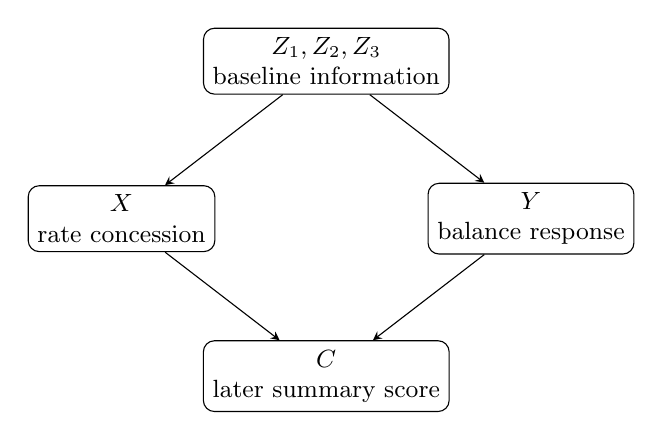
\begin{tikzpicture}[>=stealth, every node/.style={font=\small}]
\node[draw,rounded corners,align=center] (z) at (0,2) {$Z_1,Z_2,Z_3$\\baseline information};
\node[draw,rounded corners,align=center] (x) at (-2.6,0) {$X$\\rate concession};
\node[draw,rounded corners,align=center] (y) at (2.6,0) {$Y$\\balance response};
\node[draw,rounded corners,align=center] (c) at (0,-2) {$C$\\later summary score};
\draw[->] (z)--(x);\draw[->] (z)--(y);
\draw[->] (x)--(c);\draw[->] (y)--(c);
\end{tikzpicture}
\caption{Each baseline factor points to both $X$ and $Y$; the box groups the
three factors for readability. There is no causal arrow from $X$ to $Y$ in
this constructed example. Conditioning on their later common consequence
$C$ nevertheless makes their residuals associated.}
\label{repair29:collider}
\end{figure}

Let all six inputs $Z_1,Z_2,Z_3,\varepsilon_X,\varepsilon_Y,\varepsilon_C$
be mutually independent standard normal variables. The structural equations
are
\begin{align}
X&=Z_1+Z_2+Z_3+\varepsilon_X,\\
Y&=Z_1+Z_2+Z_3+\varepsilon_Y,\\
C&=X+Y+\varepsilon_C.
\end{align}
An intervention replacing the first equation changes $X$ and then $C$.
It leaves the equation for $Y$ unchanged. The mean effect on $Y$ is therefore
zero. In contrast, the unadjusted regression coefficient of $Y$ on $X$ is
$\operatorname{Cov}(X,Y)/\operatorname{Var}(X)=3/4$: common causes produce a
positive association without a treatment effect.

After adjusting for the three baseline factors, the residuals are
$X^*=\varepsilon_X$, $Y^*=\varepsilon_Y$ and
$C^*=\varepsilon_X+\varepsilon_Y+\varepsilon_C$. Thus
$\operatorname{Cov}(X^*,Y^*)=0$, and Gaussianity makes this conditional
independence. Adding the later score to the adjustment gives instead
\begin{align}
\operatorname{Cov}(X,Y\mid Z_1,Z_2,Z_3,C)
 &=0-\frac{\operatorname{Cov}(X^*,C^*)
                 \operatorname{Cov}(C^*,Y^*)}{\operatorname{Var}(C^*)}
 =-\frac13,\\
\operatorname{Var}(X\mid Z_1,Z_2,Z_3,C)&=1-\frac13=\frac23.
\end{align}
The corresponding regression coefficient is $(-1/3)/(2/3)=-1/2$.
Among customers with the same later score, a larger concession must tend
to accompany a smaller balance residual. This restriction is created by the
comparison, not by the intervention. The same structural law therefore has
a true effect of zero, an unadjusted slope of $3/4$, a baseline-adjusted slope
of zero and an overadjusted slope of $-1/2$.

Exact rational arithmetic verifies that none of the eleven conditioning sets
of size at most two separates $X$ and $Y$. At depth three the baseline set
does separate them, but the union of their neighbours also contains $C$.
The all-neighbour screen sees the nonzero conditional covariance and prevents
the valid subset from being tested. Four- and five-common-cause versions
produce the same $-1/2$ overadjusted slope, while their unadjusted slopes are
$4/5$ and $5/6$. The counterexample is consequently not peculiar to a single
three-factor covariance matrix.

For a bank, the immediate remedy is to respect the information clock and
preserve the distinction between adjustment candidates and later outcomes.
Removing the later score from the baseline information is economically
justified here. A general-purpose search still needs to handle colliders
correctly when they belong to its stated graph. The calculation does not
justify deleting inconvenient variables until a desired answer appears.

\subsection{Compare the repaired search on the same questions}

Both project searches start from the same complete undirected graph. At
each depth they test the same distinct subsets from each endpoint's
neighbourhood and remove separated pairs at the end of the depth. One search
adds the inspected screening rule; the repaired search does not. Freezing
neighbourhoods within a depth makes the comparison insensitive to the order
in which links are removed during that depth. Identical subsets available
from both endpoints are counted once in both implementations.

The principal oracle constructs the ancestral graph of the queried pair
and conditioning set, joins parents of each included node, and checks
connectivity after deleting conditioned nodes. An independently written
oracle enumerates paths and checks whether each internal node blocks or
opens the path. They agree on all conditioning queries for every ordered
four-variable graph and all queries used in the constructed witness family:
3,090 comparisons in total. The generating graph supplies the separate
reference skeleton. These checks address errors in the experiment itself;
they are not a theorem about every graph or a calibration study for noisy data.

\begin{table}[htbp]
\centering\small
\begin{tabular}{lrrrr}
\toprule
Declared case group & Cases & Full errors & Screen errors & Depth-2 errors\\
\midrule
All ordered graphs, 2--5 variables & 1,098 & 0 & 0 & 66\\
Seeded six-variable graphs & 256 & 0 & 22 & 72\\
Common-cause witness family & 3 & 0 & 3 & 3\\
Relabelled six-variable witness & 24 & 0 & 24 & 24\\
\bottomrule
\end{tabular}
\caption{An error means the returned undirected skeleton differs from the
generating skeleton. Every query uses an exact population independence
oracle. The seeded graphs use four declared edge probabilities; these
frequencies are descriptive of this finite suite, not estimates of failures
among banking applications. Relabellings are checks of the same witness,
not independent scientific replications.}
\label{repair29:results}
\end{table}

The full search recovers the reference skeleton on all 1,381 declared cases.
The screened search fails on 49, including 22 of the 256 seeded six-variable
graphs and all witness cases. Its success on every graph with at most five
variables would therefore give false reassurance if small examples alone
were used to judge it. The repair removes the observed logical obstruction
within the tested scope. It supplies no evidence that a selected finite-sample
test is sufficiently accurate, or that the data are faithful to a causal graph.

Counting independence requests reveals the cost of the shortcut. On the
ordered two-to-five-variable group, screening makes 46,856 requests versus
43,090 for full search: the extra screening step costs more than it saves.
On the seeded six-variable group it makes 25,651 requests versus 29,483,
but returns 22 wrong skeletons. These are calls in matched project searches,
not measurements of elapsed time in the Java product. An implementation
choice should compare accuracy and cost on the same declared task rather
than treat fewer calls as a scientific improvement.

\subsection{A computation budget should leave an honest question open}

A depth limit can be sensible when there are many variables. It changes
what has been learned. In the depth-two comparison, 165 cases return a
skeleton different from the generating one. Each of those cases is explicitly
marked incomplete because larger neighbouring conditioning sets remain
untested. The same warning also appears in some cases whose returned
skeleton happens to be correct. A stopping rule cannot know that fortunate
outcome without doing the omitted work or imposing additional justified
restrictions.

For the hypothetical bank, a retained $X$--$Y$ link is therefore insufficient
grounds to value a repricing policy. A report should distinguish the
independences actually found, the remaining candidate links, and the
search that was left unfinished. A graph skeleton alone also leaves arrow
directions and intervention effects unresolved. The economic next step may
be stronger pre-decision measurement, a justified model restriction or an
experiment; another graph-search heuristic need not supply the missing fact.

The proposal recommendation is to retain full subset search as the declared
reference and exclude this all-neighbour freezing rule for a general
Gaussian-oracle adaptation. A bounded implementation should return an
incomplete-search result when it stops early. Native package comparisons,
sampling calibration, orientation, prior-knowledge enforcement and endpoint
preservation remain distinct prototype tests. This result closes a specific
repair question and sharpens the software selection; it does not close the
complete Java survey or establish a bank-ready discovery engine. The next chapter asks a prior question for any such search: whether the recorded variables and customer identities faithfully represent the economic observations whose relationships are being learned.
